%%%%%%%%%%%%%%%%%%%%%%%%%%%%%%%%%%%%%%%%%
% Short Sectioned Assignment
% LaTeX Template
% Version 1.0 (5/5/12)
%
% This template has been downloaded from:
% http://www.LaTeXTemplates.com
%
% Original author:
% Frits Wenneker (http://www.howtotex.com)
%
% License:
% CC BY-NC-SA 3.0 (http://creativecommons.org/licenses/by-nc-sa/3.0/)
%
%%%%%%%%%%%%%%%%%%%%%%%%%%%%%%%%%%%%%%%%%

%----------------------------------------------------------------------------------------
%	PACKAGES AND OTHER DOCUMENT CONFIGURATIONS
%----------------------------------------------------------------------------------------

\documentclass[paper=a4, fontsize=11pt]{scrartcl} % A4 paper and 11pt font size

\usepackage[T1]{fontenc} % Use 8-bit encoding that has 256 glyphs
%\usepackage{fourier} % Use the Adobe Utopia font for the document - comment this line to return to the LaTeX default
\usepackage[english]{babel} % English language/hyphenation
\usepackage{amsmath,amsfonts,amsthm} % Math packages

\usepackage{lipsum} % Used for inserting dummy 'Lorem ipsum' text into the template

\usepackage{graphicx}
\usepackage{caption}
\usepackage{subcaption}

\usepackage{sectsty} % Allows customizing section commands
\allsectionsfont{\centering \normalfont\scshape} % Make all sections centered, the default font and small caps

\usepackage{fancyhdr} % Custom headers and footers
\pagestyle{fancyplain} % Makes all pages in the document conform to the custom headers and footers
\fancyhead{} % No page header - if you want one, create it in the same way as the footers below
\fancyfoot[L]{} % Empty left footer
\fancyfoot[C]{} % Empty center footer
\fancyfoot[R]{\thepage} % Page numbering for right footer
\renewcommand{\headrulewidth}{0pt} % Remove header underlines
\renewcommand{\footrulewidth}{0pt} % Remove footer underlines
\setlength{\headheight}{13.6pt} % Customize the height of the header

\numberwithin{equation}{section} % Number equations within sections (i.e. 1.1, 1.2, 2.1, 2.2 instead of 1, 2, 3, 4)
\numberwithin{figure}{section} % Number figures within sections (i.e. 1.1, 1.2, 2.1, 2.2 instead of 1, 2, 3, 4)
\numberwithin{table}{section} % Number tables within sections (i.e. 1.1, 1.2, 2.1, 2.2 instead of 1, 2, 3, 4)

\setlength\parindent{0pt} % Removes all indentation from paragraphs - comment this line for an assignment with lots of text

%----------------------------------------------------------------------------------------
%	TITLE SECTION
%----------------------------------------------------------------------------------------

\newcommand{\horrule}[1]{\rule{\linewidth}{#1}} % Create horizontal rule command with 1 argument of height

\title{	
\normalfont \normalsize 
\textsc{ETH Zurich, D-INFK} \\ [25pt] % Your university, school and/or department name(s)
\horrule{0.5pt} \\[0.4cm] % Thin top horizontal rule
\huge Computer Vision: Assignment 1 \\ % The assignment title
\horrule{2pt} \\[0.5cm] % Thick bottom horizontal rule
}

\author{Igor Pesic} % Your name

\date{\normalsize\today} % Today's date or a custom date

\begin{document}

\maketitle % Print the title

%----------------------------------------------------------------------------------------
%	PROBLEM 1
%----------------------------------------------------------------------------------------

\section{Feature extraction}


I have implemented the feature extraction step basically as described in the exercise sheet with the addition of the Gaussian blurring of the image derivatives. In order to avoid multiple for loops in MATLAB, I have precomputed the sums of the blurred  $I_{x}^2$, $I_{y}^2$ and $I_{xy}$. I chose the threshold of $0.005$ for Harris response measure. 

%------------------------------------------------

\subsection{Non-maximum suppression comparison}

In Figures \ref{fig:supr1} and \ref{fig:supr2} are the Harris corners before and after non-maximum suppression. As we can notice, when non-maximum suppression is not used, the areas of dense keypoints get even more dense and the number of total keypoints in the image increases drastically. With no suppression, the number of keypoints is around 11k and 31k for the 2 images respectively and with the suppression the number of keypoints drops to around 430 and 720 respectively.

\begin{figure}
\centering
\begin{subfigure}{.5\textwidth}
  \centering
  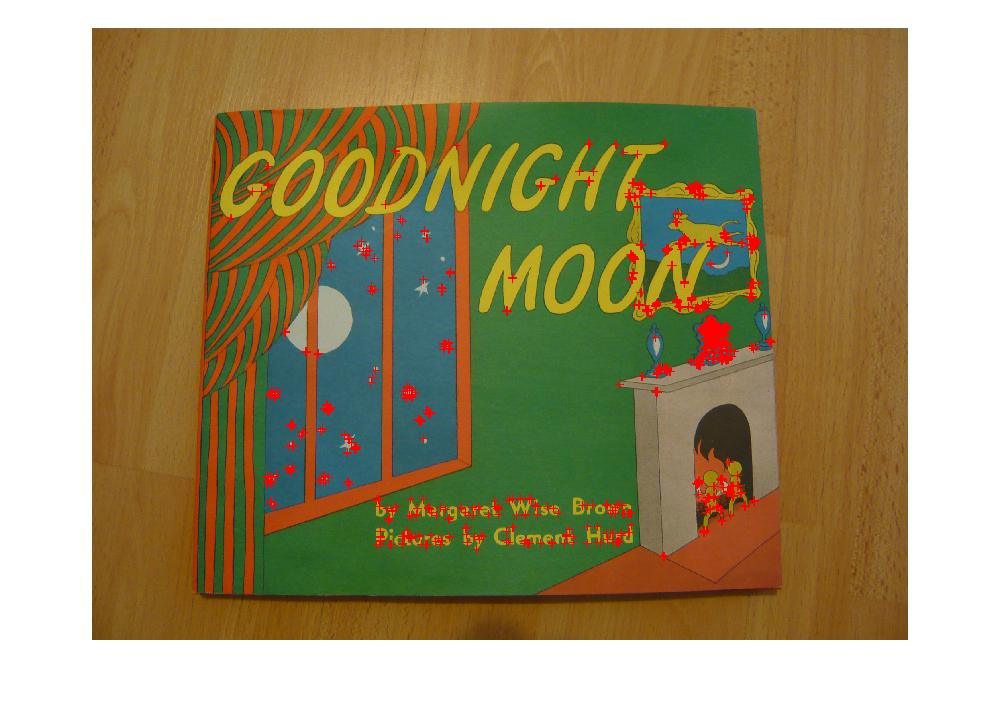
\includegraphics[width=1\linewidth]{img1_harris_no_supr.jpg}
  \caption{No suppression}
\end{subfigure}%
\begin{subfigure}{.5\textwidth}
  \centering
  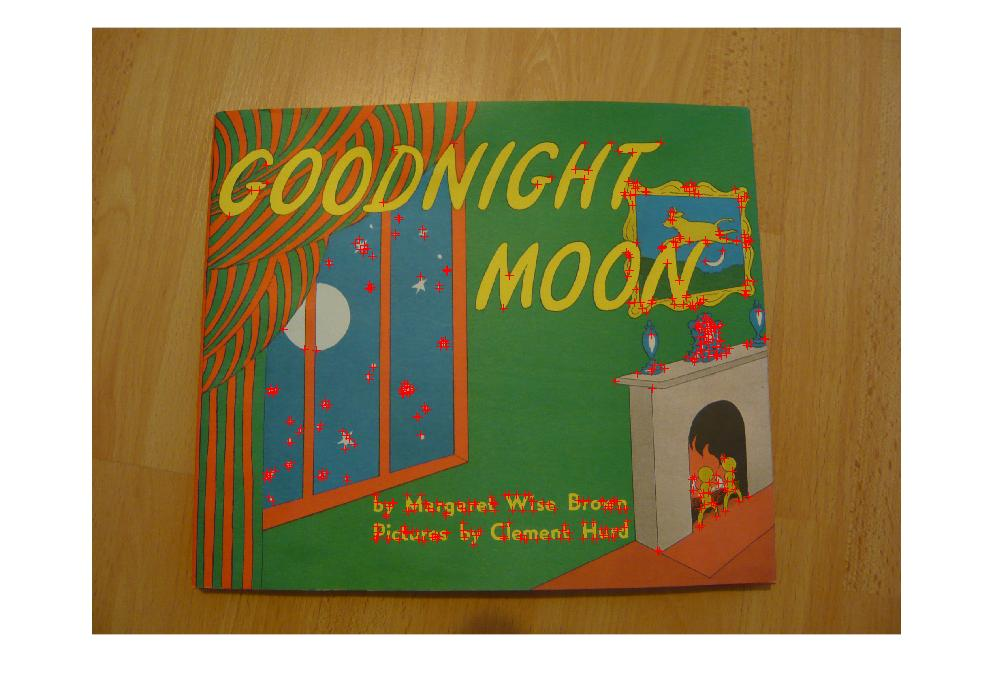
\includegraphics[width=1\linewidth]{im1_harris_corners.jpg}
  \caption{With suppression}
\end{subfigure}
\caption{Non-max. suppression compariosn for image 1}
\label{fig:supr1}
\end{figure}

\begin{figure}
\centering
\begin{subfigure}{.5\textwidth}
  \centering
  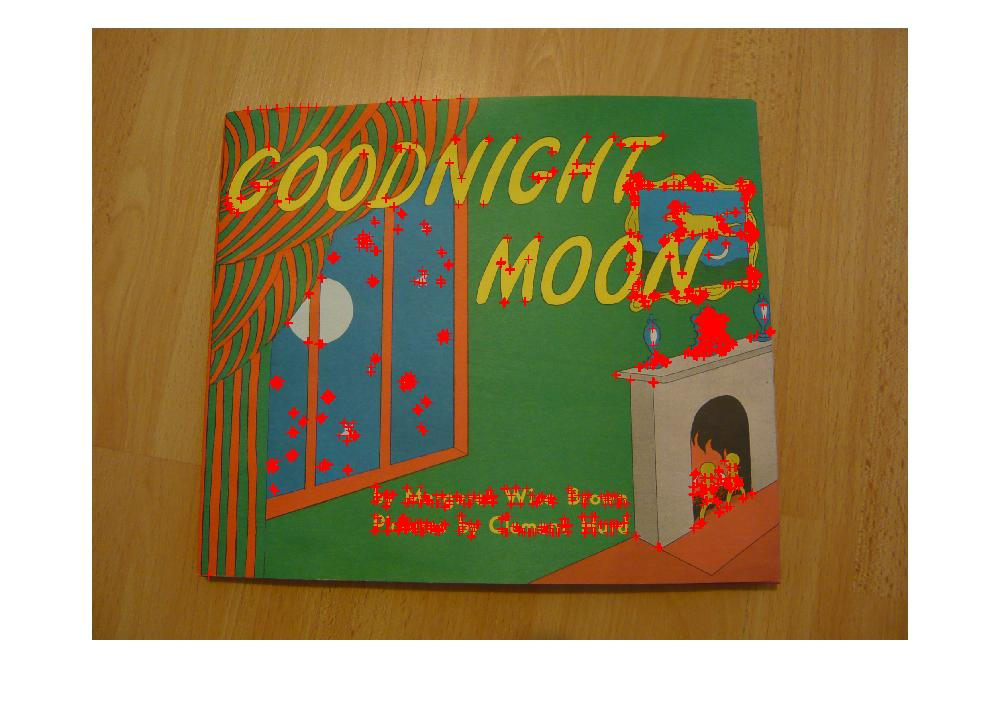
\includegraphics[width=1\linewidth]{img2_harris_no_supr.jpg}
  \caption{No suppression}
\end{subfigure}%
\begin{subfigure}{.5\textwidth}
  \centering
  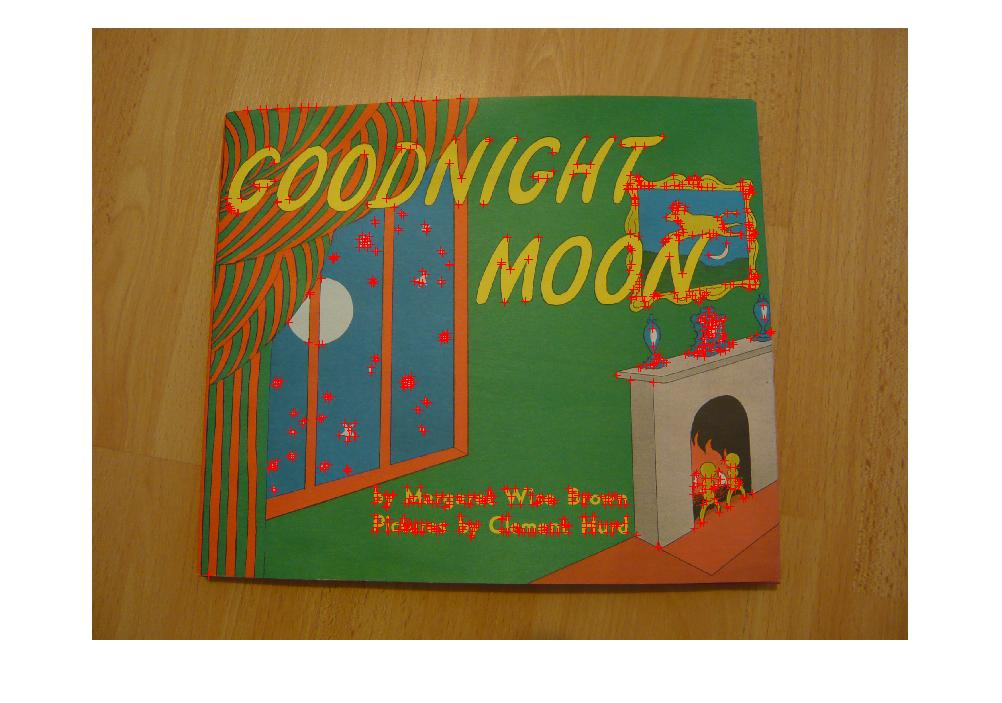
\includegraphics[width=1\linewidth]{im2_harris_corners.jpg}
  \caption{With suppression}
\end{subfigure}
\caption{Non-max. suppression compariosn for image 2}
\label{fig:supr2}
\end{figure}

%------------------------------------------------

\subsection{SIFT comparison}

I have ran the SIFT library with $PeakThresh = 0.02$ for both images. I have chosen this value empirically, so that the images are not too crowded with the keypoints. In Figures \ref{fig:sift1} and \ref{fig:sift2} are the comparisons of my implementation of Harris corner detection and the vlfeat SIFT implementation. \\
\\
I have got the feeling that SIFT has found many points that do not represent corners, but rather edges. On the other hand, Harris corner detector had way less of the key points on the edges. Nevertheless points found by SIFT are more distributed across the whole image, while Harris has failed to identify lots of points in the upper and in the left part of the image. 

\begin{figure}
\centering
\begin{subfigure}{.5\textwidth}
  \centering
  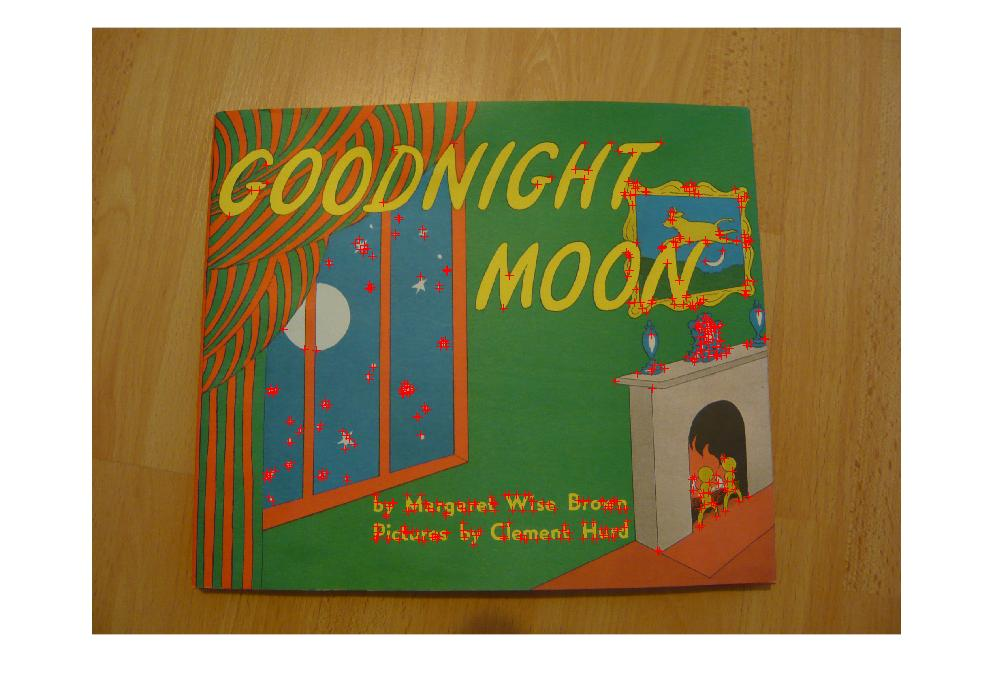
\includegraphics[width=1\linewidth]{im1_harris_corners.jpg}
  \caption{Harris}
\end{subfigure}%
\begin{subfigure}{.5\textwidth}
  \centering
  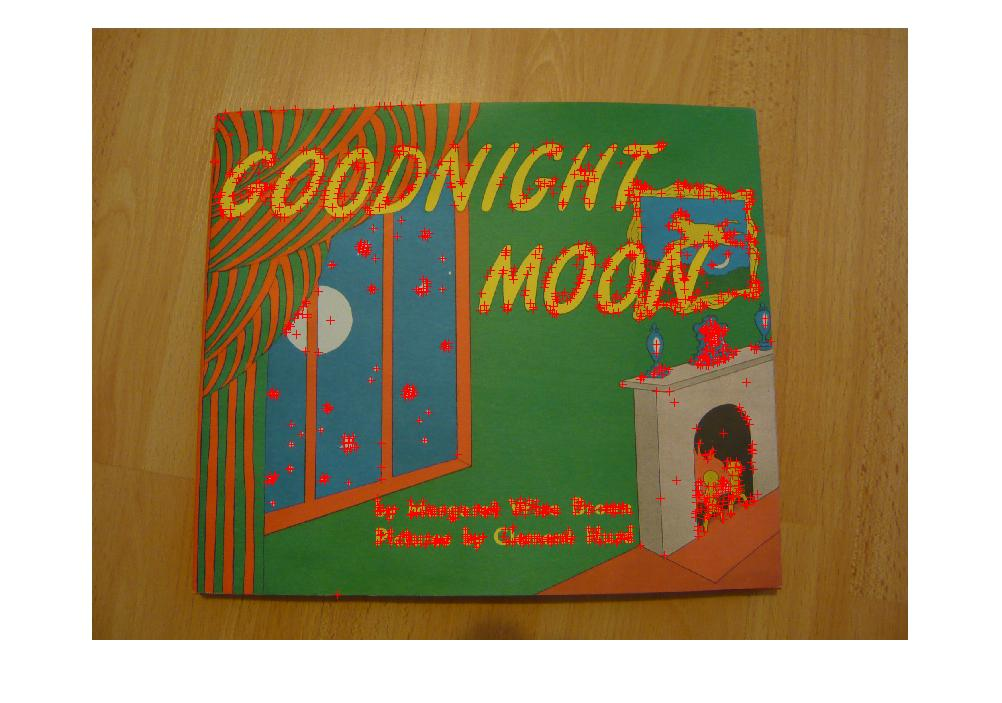
\includegraphics[width=1\linewidth]{img1_sift_corners.jpg}
  \caption{SIFT}
\end{subfigure}
\caption{Harris vs SIFT corner detection for image 1.}
\label{fig:sift1}
\end{figure}

\begin{figure}
\centering
\begin{subfigure}{.5\textwidth}
  \centering
  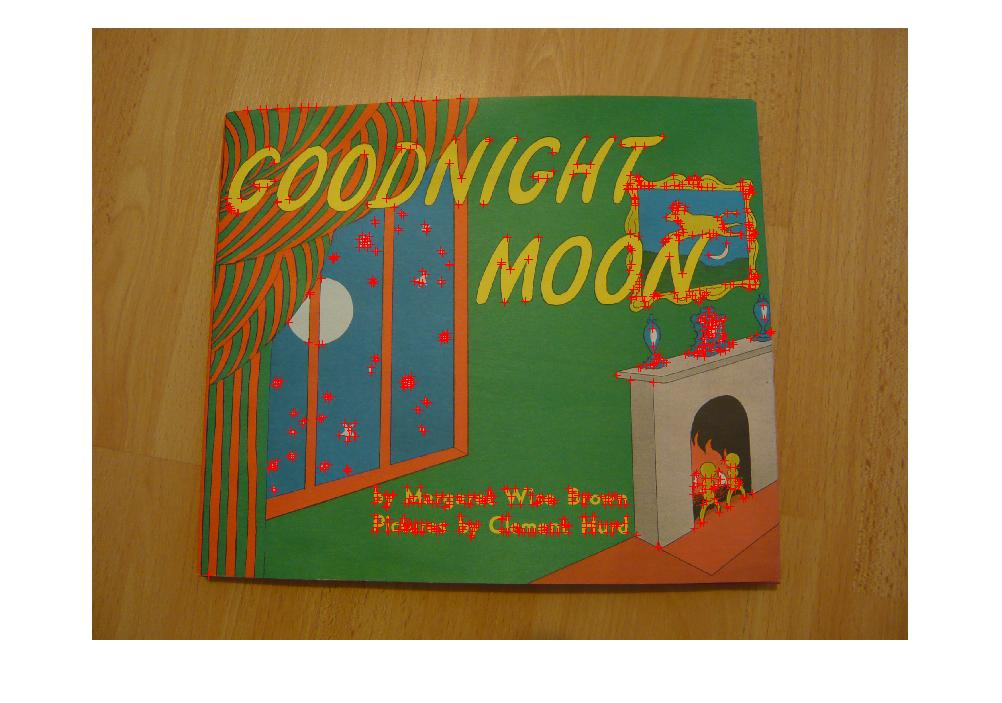
\includegraphics[width=1\linewidth]{im2_harris_corners.jpg}
  \caption{Harris}
\end{subfigure}%
\begin{subfigure}{.5\textwidth}
  \centering
  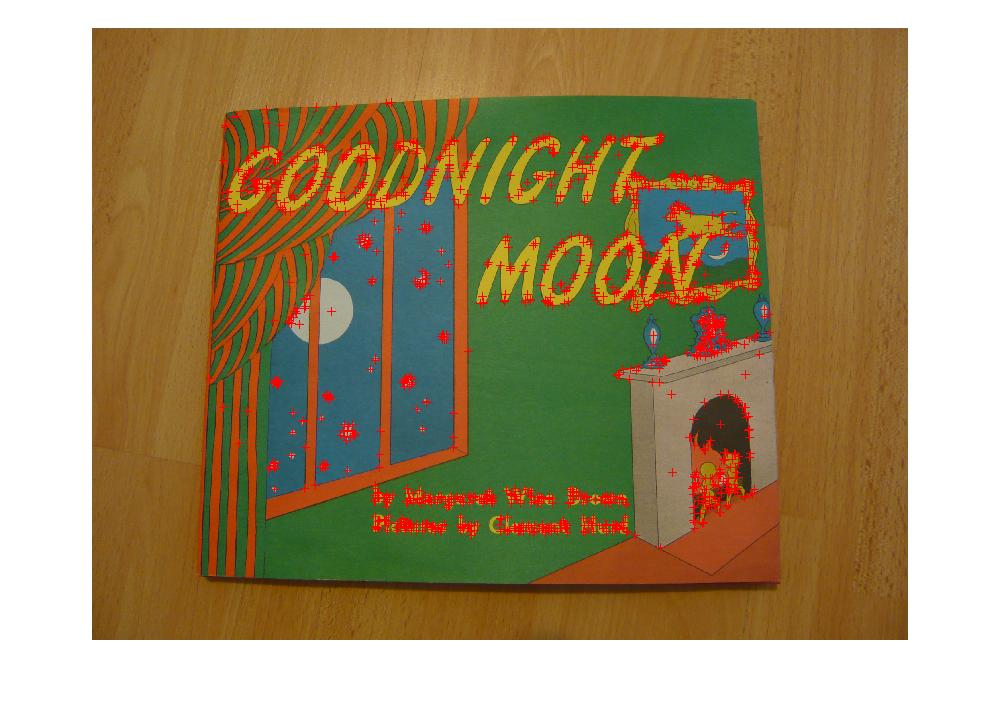
\includegraphics[width=1\linewidth]{img2_sift_corners.jpg}
  \caption{SIFT}
\end{subfigure}
\caption{Harris vs SIFT corner detection for image 2.}
\label{fig:sift2}
\end{figure}


\subsection{Feature matches}

In figures \ref{fig:match_harris} and \ref{fig:match_sift} I have plotted the matched keypoints obtained by both methods. Obviously, since SIFT has obtained more keypoints on both images, it has more matches than Harris corner detector. Also the matches of the SIFT descriptors are more accurate. On the other hand, the simple matching algorithm that I have implemented has also a pretty good accuracy with only small fraction of keypoints that are not matched correctly.

\begin{figure}
  \centering
  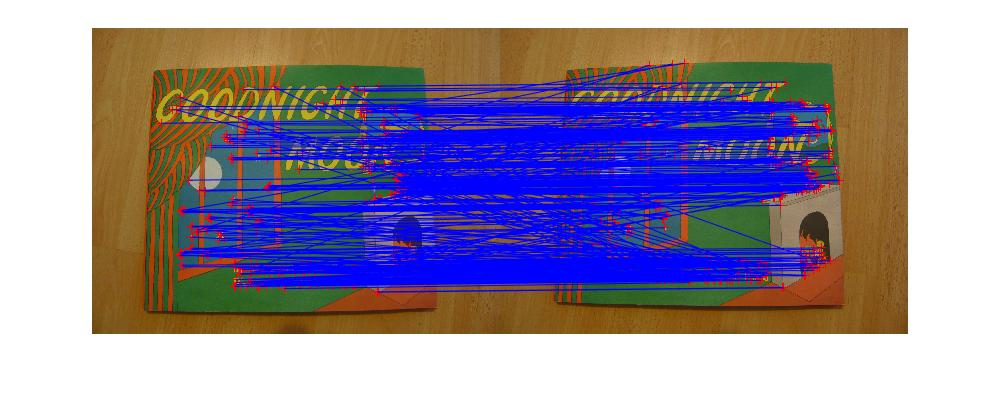
\includegraphics[width=1\linewidth]{harris_matches.jpg}
\caption{Harris matches}
\label{fig:match_harris}
\end{figure}

\begin{figure}
  \centering
  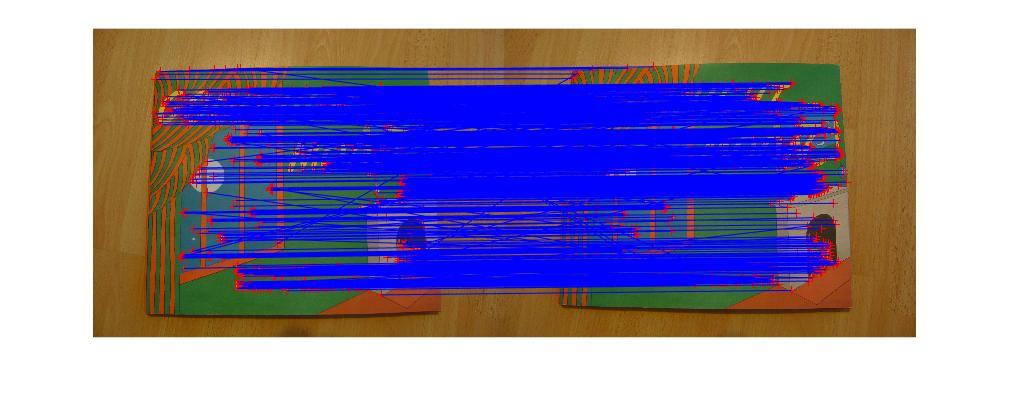
\includegraphics[width=1\linewidth]{sift_matches.jpg}
\caption{SIFT matches}
\label{fig:match_sift}
\end{figure}

\end{document}